\documentclass{beamer}

\usetheme{spensiones}
\usepackage{stata}
\usepackage{tikz, tabularx, ulem}
\usetikzlibrary{arrows, fit,positioning}

\title[{\tt parallel}]{{\tt parallel}: M\'odulo de Stata para computaci\'on en paralelo}

\author[GVY]{George Vega Yon}
\institute[SPensiones \and UAI]{Superintendencia de Pensiones \and Universidad Adolfo Ib\'a\~nez}
\def\unix1{Intel Xeon X470 (octa-core)}
\begin{document}

\frame{\maketitle}

\frame{
\frametitle{Agenda}
\tableofcontents
}

\section{Motivaci\'on}

\begin{frame}[allowframebreaks=.8]
\frametitle{Motivaci\'on}
\begin{itemize}
\item Actualmente los computadores caseros vienen con grandes capacidades computacionales.
\item CPU Multiprocesadores son el est\'andar en la industria de hoy.
\item Motivados por la industria de los video juegos, los fabricantes han forjado un mercado de CPU de bajo costo con potencia de procesamiento comparables a las de un peque\~no supercomputador (Aldrich, Fern\'andez-Villaverde, Ronald Gallant \& Rubio-Ram\'irez, 2011).
\item De la misma forma la disponiblidad de datos ha aumentado significativamente ({\it big-data})
\item Recursos que, a pesar de estar disponibles para investigadores y {\it hacedores} de pol\'itcas p\'ublicas no han sido muy explotados.
\item Varias trabas a esto han sido asuntos involucrando privacidad, administraci\'on y ausencia de herramientas computacionales para poder manejar estos grandes vol\'umenes de datos (King 2011).
\item {\tt parallel} apunta a contribuir en este \'ultimo asunto.
\end{itemize}
\end{frame}

\section{Computaci\'on en Paralelo}
\begin{frame}[allowframebreaks=.8]
\frametitle{Computaci\'on en Paralelo}

\begin{itemize}
\item En t\'erminos sencillos, computaci\'on en paralelo es el uso simult\'aneo de multiples recursos computacionales para resolver problemas computacionales (Barney, 2012).
\item Computaci\'on en paralelo puede tomar lugar en distintos niveles desde (a) nivel de bit, (b) a nivel de instrucci\'on, (c) a nivel de datos y hasta (d) nivel de tareas.
\item {\tt parallel} utiliza paralelismo de datos cual b\'asicamente consiste en repetir una tarea de forma simult\'anea sobre grupos o bloques independientes de datos.
\item Haciendo uso de computaci\'on en paralelo es posible disminuir de manera dr\'astica el tiempo requerido para completar un problema computacional.
\item Esto es esencialmente importante para diversas \'areas de las ciencias tales como econom\'ia emp\'irica, estad\'istica, econometr\'ia y epidemiolog\'ia, dado que de esta forma es posible implementar algoritmos caracterizados por un gran n\'umero de c\'alculos o, en el caso de Stata, interpretaci\'on de c\'odigo tales como bucles.
\end{itemize}

\end{frame}

\section{{\tt parallel}: Acelerando los tiempos de respuesta de la administraci\'on p\'ublica}

\begin{frame}[allowframebreaks=.8]
\frametitle{Qu\'e es {\tt parallel}?}

\begin{itemize}
\item Inspirado en la librer\'ia del paquete estad\'istico {\tt R} ``snow''
\item Dise\~nado para ser utilizado con computadores multinucleo (dualcore, quadcore, etc.)
\item {\tt parallel} implementa paralelismo de datos para aumentar dr\'asticamente la velocidad de c\'alculo
\item Dividiendo la tarea en bloques de datos (clusters) {\tt parallel} repite \'ordenes de manera simult\'anea sobre estos.
\item Disminuir tiempos de c\'alculo varias veces dependiendo del n\'umero de procesadores con que el ordenador cuente. Así el tener 8 procesadores (como en la Superintendencia de Pensiones) puede implicar dismunir el tiempo de c\'alculo en 8 (o m\'as) veces.
\item Ya implementado en algunos modelos de la Divisi\'on de Estudios de la Superintendencia de Pensiones, ha logrado hacer que complejos modelos pasen de tardar m\'as de una semana en correr a menos de dos días.
\item El producto es totalmente replicable ya que:
\begin{itemize}
\item Por como fue dise\~nado, no es necesario que el usuario posea un conocimiento profundo en programaci\'on estad\'istica.
\item El c\'odigo es abierto y ha sido publicado en el repositorio de la Universidad de Boston \url{http://ideas.repec.org/c/boc/bocode/s457527.html}
\item Se adapta a las distintas versiones de Stata (desde la b\'asica hasta la m\'as costosa).
\item Se encuentra publicado y documentado completamente en ingl\'es.
\end{itemize}
\end{itemize}

\end{frame}

\section{C\'omo funciona?}

\begin{frame}
\frametitle{C\'omo funciona?}
\begin{figure}
\centering
\scalebox{.65}{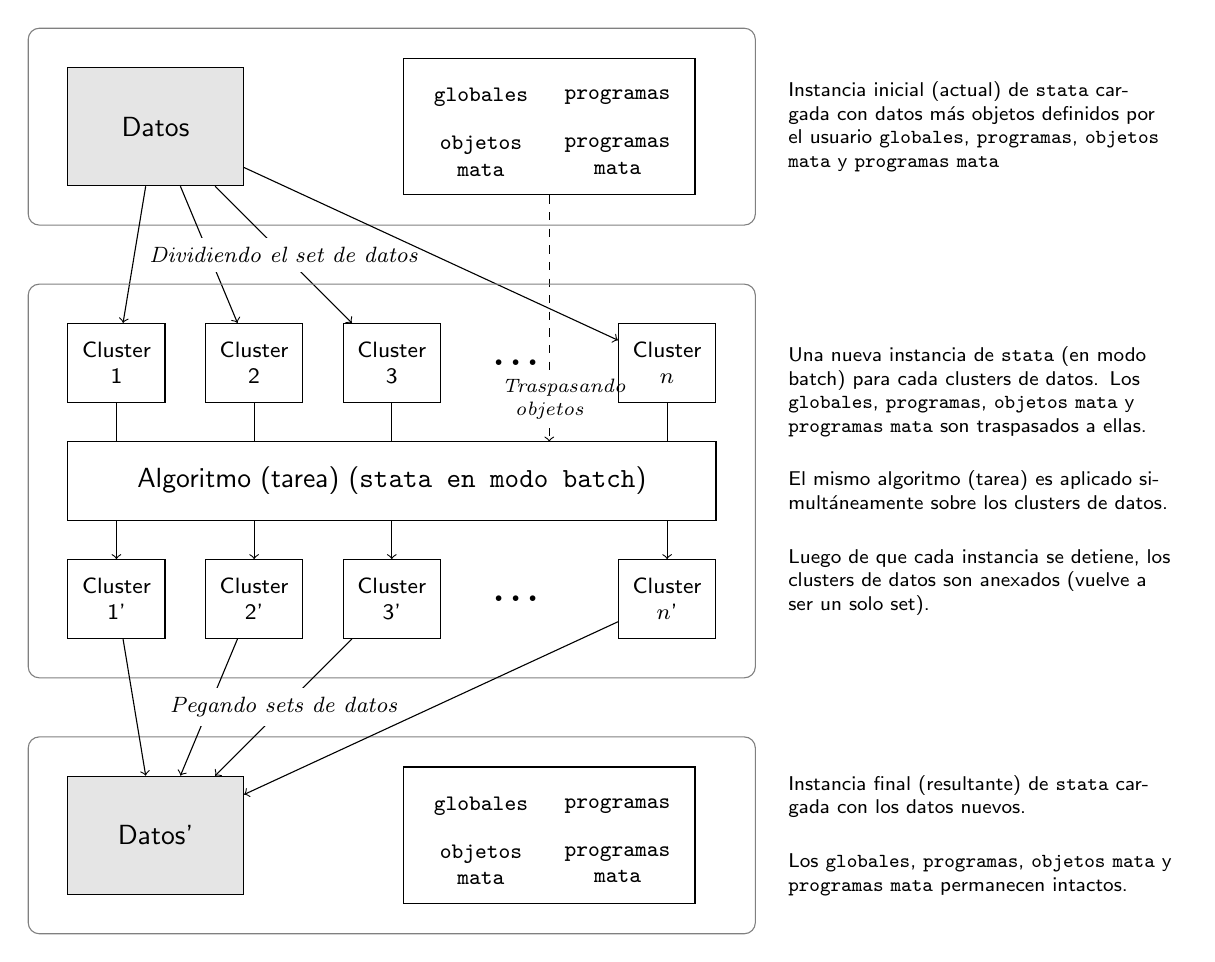
\begin{tikzpicture}[
	every node/.style={node distance=.5cm and .5cm, font=\sffamily}, 
	datablock/.style={rectangle, draw, fill=black!10, text width=2cm, minimum height=1.5cm, text badly centered},
	cluster/.style={rectangle, draw,text width=1cm, text badly centered, minimum height=1cm, font=\footnotesize\sffamily},
	explain/.style={rectangle, text width=5.5cm, align=left, font=\footnotesize\sffamily, node distance=.3, scale=.9}
	] 
	
\node [rectangle, draw=gray, text width=9cm, minimum height=2.5cm, rounded corners] (stata instance0) at (0,0) {};

% Original data
\node [datablock] (data) at (-3,0) {Datos};
\matrix [
	draw=black,
	nodes={
		rectangle, text width=1.5cm, minimum height=.75cm, 
		scale=1,
		font=\tt\footnotesize, text badly centered}, column sep=0, row sep=0
	] (others) at (2,0) {
	\node {globales};& \node {programas}; \\
	\node {objetos mata}; & \node {programas mata}; \\
};

% Data clusters
\node [cluster] (cluster3) at (0,-3) {Cluster 3};
\node [cluster, left=of cluster3] (cluster2) {Cluster 2};
\node [cluster, left=of cluster2] (cluster1) {Cluster 1};
\node [rectangle, right=of cluster3, text width=1cm, font=\Huge] (threepoints) {...};
\node [cluster, right=of threepoints,text badly centered] (clustern) {Cluster $n$};

% Splitting
\draw[->] (data) -- (cluster1);
\draw[->] (data) -- (cluster2);
\draw[->] (data) -- node [fill=white, font=\footnotesize\it] {Dividiendo el set de datos} (cluster3);
\draw[->] (data) -- (clustern);

\draw[->, dashed] (others) -- node [fill=white, font=\scriptsize\it, below=.65cm, text width=1.2cm, minimum height=.7cm,text badly centered] {Traspasando objetos} (2,-4);

% Procesed clusters
\node [cluster] (cluster3p) at (0,-6) {Cluster 3'};
\node [cluster, left=of cluster3p] (cluster2p) {Cluster 2'};
\node [cluster, left=of cluster2p] (cluster1p) {Cluster 1'};
\node [rectangle, right=of cluster3p, text width=1cm, font=\Huge] (threepointsp) {...};
\node [cluster, right=of threepointsp,text badly centered] (clusternp) {Cluster $n$'};

\draw[->] (cluster1) -- (cluster1p);
\draw[->] (cluster2) -- (cluster2p);
\draw[->] (cluster3) -- (cluster3p);
\draw[->] (clustern) -- (clusternp);

% Task
\node [rectangle, draw=gray, text width=9cm, minimum height=5cm, rounded corners] (stata batch) at (0,-4.5) {};
\node [rectangle, fill=white, draw, text width=8cm, text badly centered,minimum height=1cm] (task) at (0,-4.5) {Algoritmo (tarea) (\texttt{stata en modo batch})};

% Result
\node [rectangle, draw=gray, text width=9cm, minimum height=2.5cm, rounded corners] (stata instance1) at (0,-9) {};
\node [datablock] (datap) at (-3,-9) {Datos'};
\matrix [
	draw=black,
	nodes={
		rectangle, text width=1.5cm, minimum height=.75cm, 
		scale=1,
		font=\tt\footnotesize, text badly centered}, column sep=0, row sep=0
	] (othersp) at (2,-9) {
	\node {globales};& \node {programas}; \\
	\node {objetos mata}; & \node {programas mata}; \\
};

\draw[->] (cluster1p) -- (datap);
\draw[->] (cluster2p) -- (datap);
\draw[->] (cluster3p) -- node [fill=white, font=\footnotesize\it] {Pegando sets de datos} (datap);
\draw[->] (clusternp) -- (datap);

% Text
\node [explain, right=of stata instance0] {Instancia inicial (actual) de {\tt stata} cargada con datos m\'as objetos definidos por el usuario {\tt globales}, {\tt programas}, {\tt objetos mata} y {\tt programas mata}};

\node [explain, right=of stata batch] {Una nueva instancia de {\tt stata} (en modo batch) para cada clusters de datos. Los {\tt globales}, {\tt programas}, {\tt objetos mata} y {\tt programas mata} son traspasados a ellas.\\\bigskip El mismo algoritmo (tarea) es aplicado simult\'aneamente sobre los clusters de datos.\\\bigskip Luego de que cada instancia se detiene, los clusters de datos son anexados (vuelve a ser un solo set).};

\node [explain, right=of stata instance1] {Instancia final (resultante) de {\tt stata} cargada con los datos nuevos.\\\bigskip Los {\tt globales}, {\tt programas}, {\tt objetos mata} y {\tt programas mata} permanecen intactos.};

\end{tikzpicture}}
\end{figure}
\end{frame}

\section{Ejemplos de uso y resultados}

\begin{frame}
\frametitle{Ejemplos de uso y resultados}

\begin{itemize}
\item En lo que sigue se presentan resultados de un par de test realizados para medir las ganancias en t\'erminos de velocidad.
\item Los valores al interior de las tablas de resultados reportan tiempos en segundos.
\item Las dos primeras filas de cada tabla reportan (a) el tiempo CPU, implementaci\'on del algoritmo sin usar {\tt parallel}, y (b) el tiempo Total, tiempo que tard\'o el mismo algoritmo en ser calculado con {\tt parallel}.
\item Las \'ultimas dos filas muestran un ratio entre el tiempo CPU (no paralelo) y el Total (paralelo), donde cualquier valor mayor a 1 corresponde a una mejora utilizando {\tt parallel}.
\end{itemize}

\end{frame}


\begin{frame}
\frametitle{Ejemplos de uso y resultados}
\framesubtitle{ejercicio sencillo}

\begin{table}[!h]
\centering
\caption{Reemplazando valores de forma serial en un servidor Linux (4 clusters)\label{tab:serialreplace_linux}}
\begin{tabular}{l*{4}{c}}\hline
& \multicolumn{4}{c}{N\'umero de reemplazos} \\
& 10.000 &           100.000 &          1.000.000 &         10.000.000 \\ \hline
CPU &     0.25 &      1.79 &     17.64 &    176.16 \\
Total &     0.45 &      1.00 &      5.14 &     42.61 \\
\hspace{2mm} Preparaci\'on &     0.02 &      0.11 &      0.81 &      5.16 \\
\hspace{2mm} C\'alculo &     0.23 &      0.67 &      3.86 &     35.98 \\
\hspace{2mm} Finalizaci\'on &     0.21 &      0.23 &      0.46 &      1.47 \\
\hline Ratio (computaci\'on) &     1.13 &      2.68 &      4.57 &      4.90 \\
Ratio (total) &     0.56 &      1.79 &      3.43 &      4.13 \\
\hline
\multicolumn{5}{l}{\footnotesize Testeado sobre \unix1}
\end{tabular}
\end{table}

\end{frame}

\begin{frame}
\frametitle{Ejemplos de uso y resultados}
\framesubtitle{ejercicio m\'as complejo}

\begin{table}[!h]
\centering
\caption{Experimento de Monte Carlo en un servidor Linux}
\begin{tabular}{l*{3}{c}}\hline
& \multicolumn{3}{c}{N\'umero de Clusters} \\
& 2 &               3 &               5 \\ \hline
CPU &    40.97 &     39.01 &     36.44 \\
Total &    18.35 &     15.20 &      7.62 \\
\hspace{2mm} Preparaci\'on &     0.11 &      0.11 &      0.12 \\
\hspace{2mm} C\'alculo &    18.13 &     14.99 &      7.41 \\
\hspace{2mm} Finalizaci\'on &     0.10 &      0.10 &      0.10 \\
\hline Ratio (computaci\'on) &     2.26 &      2.60 &      4.92 \\
Ratio (total) &     2.23 &      2.57 &      4.78 \\
\hline
\multicolumn{4}{c}{\footnotesize Testeado sobre \unix1}
\end{tabular}
\end{table}

\end{frame}

\section{Sintaxis}

\begin{frame}
\frametitle{Sintaxis}
\footnotesize
\begin{semiverbatim}
{\bf parallel setclusters} {\it \#}  [, \uline{f}orce] \pause

{\bf parallel do} {\it \color{blue} filename}

\hspace{1cm} [, by({\it \color{blue} varlist}) \uline{f}orce \uline{k}eep \uline{keepl}ast \uline{p}rograms \uline{m}ata 

\hspace{1cm} \uline{nog}lobal \uline{s}eeds({\it \color{blue} numlist}) \uline{nod}ata] \pause

{\bf parallel}  [, by({\it \color{blue} varlist}) \uline{f}orce \uline{k}eep \uline{keepl}ast \uline{p}rograms \uline{m}ata 

\hspace{1cm} \uline{nog}lobal \uline{s}eeds({\it \color{blue} numlist}) \uline{nod}ata]:  {\it stata\_cmd}
\end{semiverbatim}
\end{frame}


\section{Ejemplos}

\begin{frame}
\frametitle{Ejemplos}\framesubtitle{setup}
\begin{stlog}
. sysuse bplong.dta
(fictional blood-pressure data)
{\smallskip}
. sort patient
{\smallskip}
. parallel setclusters 4
N Clusters: 4
Stata dir:  /usr/local/stata12/stata-se
{\smallskip}

\end{stlog}

\end{frame}

\begin{frame}
\frametitle{Ejemplos}\framesubtitle{egen by}
\footnotesize
\begin{stlog}
. bysort patient: egen max_bp = max(bp)
{\smallskip}
. parallel, by(patient) nog: by patient: egen max_bp_pll = max(bp)
Parallel Computing with Stata (by GVY)
Clusters: 4
ID: gwvf2ap6d3
{\smallskip}
[1] 29870
Stata instances PID:
[1] 29880
[2] 29881
[3] 29882
[4] 29883
{\sltt{cluster 1}} has finished without any error...
{\sltt{cluster 2}} has finished without any error...
{\sltt{cluster 3}} has finished without any error...
{\sltt{cluster 4}} has finished without any error...
{\smallskip}
. summ max_bp*
{\smallskip}
    Variable {\VBAR}       Obs        Mean    Std. Dev.       Min        Max
\HLI{13}{\PLUS}\HLI{56}
      max_bp {\VBAR}       240    160.8333    11.56993        138        185
  max_bp_pll {\VBAR}       240    160.8333    11.56993        138        185
{\smallskip}

\end{stlog}

\end{frame}

\begin{frame}[allowframebreaks=1]
\frametitle{Ejemplos}\framesubtitle{reshape}
\begin{stlog}
. qui reshape wide bp max_bp*, i(patient) j(when)
{\smallskip}
. summ 
{\smallskip}
    Variable {\VBAR}       Obs        Mean    Std. Dev.       Min        Max
\HLI{13}{\PLUS}\HLI{56}
     patient {\VBAR}       120        60.5    34.78505          1        120
         bp1 {\VBAR}       120      156.45    11.38985        138        185
     max_bp1 {\VBAR}       120    160.8333    11.59421        138        185
 max_bp_pll1 {\VBAR}       120    160.8333    11.59421        138        185
         bp2 {\VBAR}       120    151.3583    14.17762        125        185
\HLI{13}{\PLUS}\HLI{56}
     max_bp2 {\VBAR}       120    160.8333    11.59421        138        185
 max_bp_pll2 {\VBAR}       120    160.8333    11.59421        138        185
         sex {\VBAR}       120          .5    .5020964          0          1
      agegrp {\VBAR}       120           2    .8199201          1          3
{\smallskip}
. qui reshape long
{\smallskip}
. qui parallel, by(patient) f nog: reshape wide bp max_bp*, i(patient) j(when)
{\smallskip}
. return list
{\smallskip}
scalars:
              r(pll_n) =  4
         r(pll_t_fini) =  .003
         r(pll_t_calc) =  .323
         r(pll_t_setu) =  0
         r(pll_t_reps) =  1
           r(pll_errs) =  0
{\smallskip}
macros:
             r(pll_id) : "r1c9jesifd"
            r(pll_dir) : "/u1/users/estudios/investigacion/george/comandos_paqu
> etes_librerias/stata/parallel"
{\smallskip}
. summ
{\smallskip}
    Variable {\VBAR}       Obs        Mean    Std. Dev.       Min        Max
\HLI{13}{\PLUS}\HLI{56}
     patient {\VBAR}       120        60.5    34.78505          1        120
         bp1 {\VBAR}       120      156.45    11.38985        138        185
     max_bp1 {\VBAR}       120    160.8333    11.59421        138        185
 max_bp_pll1 {\VBAR}       120    160.8333    11.59421        138        185
         bp2 {\VBAR}       120    151.3583    14.17762        125        185
\HLI{13}{\PLUS}\HLI{56}
     max_bp2 {\VBAR}       120    160.8333    11.59421        138        185
 max_bp_pll2 {\VBAR}       120    160.8333    11.59421        138        185
         sex {\VBAR}       120          .5    .5020964          0          1
      agegrp {\VBAR}       120           2    .8199201          1          3
{\smallskip}

\end{stlog}

\end{frame}

\section{Aplicaciones e Implicancias}

\begin{frame}
\frametitle{Aplicaciones e Implicancias}

\begin{itemize}
\item Al conocimiento del autor, {\tt parallel} es el primer paquete de computaci\'on en paralelo escrito para Stata.
\item Gracias a la existencia de este m\'odulo, gobiernos y usuarios del mundo podr\'an ahorrarse miles de dolares en licencias al evitar comprar la licencia de Stata/MP (multiprocesadores)\footnote{La licencia de 8 procesadores para 20 usuarios cuesta unos U\$28.000.}.
\item Como directa implicancia permite a investigadores, analistas y ``hacedores'' de pol\'itica p\'ublica:
\begin{itemize}
\item Implementar algoritmos m\'as complejos
\item Aumentar significativamente su productividad
\item Sacar el m\'aximo provecho de los recursos computacionales modernos
\item Y, por lo tanto, generar mejores pol\'itcas impactando tanto en el dise\~no como en la evaluaci\'on.
\end{itemize}
\end{itemize}

\end{frame}

\frame{\maketitle}

\end{document}